\section{Per-patient scoring}
\label{sec:scoring}

A map is only useful if every patient can be placed on it. Because fitting and scoring separate cleanly under
the marginalized model (Chapter~\ref{sec:estimation}), the map is fit \emph{once} and then every patient is
\emph{projected} onto it: for a fixed posterior draw, a patient's coordinate on a continuous-anchored dimension
is the Gaussian conditional $z_i\mid x_{i,\Obs_i}$ with mean $A_i^{-1}b_i$ and precision $A_i$ --- the same
$A_i,b_i$ that defined the likelihood. The explicit dimensions (suicidality, developmental, substance) are read
from their latent $f_e$ on the fit sub-sample. All $9{,}013$ patients receive, per dimension, a posterior
\textbf{mean}, \textbf{SD}, and \textbf{HDI}, the \textbf{number of observed home indicators}, and a
\textbf{reliability tier}, all oriented so higher $=$ more burden.

\begin{definitionbox}[Coordinates carry honest uncertainty --- a GPS with error bars]
A patient scored from six observed cognition tasks is located precisely; a patient with none is placed at the
population prior with a wide error bar. Treating those two as equally measured is exactly the mistake the
reliability tier prevents. A coordinate is \emph{well-characterised} ($\ge 3$ observed home indicators),
\emph{partial} ($1$--$2$), or \emph{prior-dominated} ($0$, i.e.\ informed only by the prior and by correlated
dimensions).
\end{definitionbox}

The tiers expose coverage honestly (Figure~\ref{fig:reliability}). $G$ is well-characterised for almost
everyone (functioning is near-universally recorded). Cognition is \emph{prior-dominated for $2{,}506$ patients}
who had no cognitive testing --- their cognition coordinate is a prior-plus-correlation guess, and is flagged
as such. Most starkly, \textbf{mania is \emph{partial} for every patient}: with only two indicators
(YMRS, Altman) it can never reach the $\ge 3$ ``well'' tier, so it is never reported as well-characterised ---
a built-in humility about a thin axis.

\begin{figure}[h]\centering
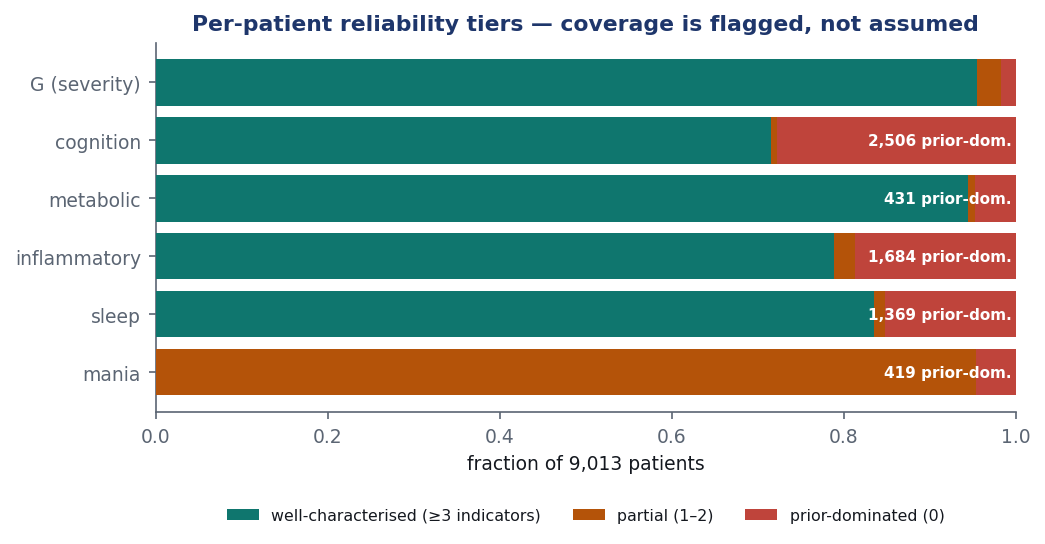
\includegraphics[width=0.82\linewidth]{figures/fig_reliability.png}
\caption{Per-patient reliability by continuous-anchored dimension: the fraction of the $9{,}013$ patients that
are well-characterised ($\ge 3$ observed home indicators), partial ($1$--$2$), or prior-dominated ($0$).
Coverage is \emph{flagged}, not assumed away --- cognition is prior-dominated for the $2{,}506$ untested
patients, and mania (only two indicators) is partial for everyone.}
\label{fig:reliability}
\end{figure}

\begin{caveatbox}[Uncertainty must propagate to the stratification]
The scores are a distribution, not a point. A stratification that hard-assigns patients to clusters on the
posterior means would discard exactly the information these tiers encode --- a prior-dominated cognition score
is not evidence of average cognition, only of \emph{absent measurement}. The per-patient SD/HDI and tier are
carried forward so downstream decision regions can down-weight or abstain where a coordinate is unreliable.
Two refinements remain: full-$N$ projection of the non-Gaussian block (a logistic/count conditional,
not Gaussian; the explicit scores are currently on the fit sub-sample), and a hurdle likelihood for
\code{isf09a} if its count precision is needed.
\end{caveatbox}
